\documentclass{article}

% Empleamos la plantilla oficial de NeurIPS 2026 en formato preprint para el reporte
\usepackage[preprint]{neurips_2026}

% --- Paquetes ---
\usepackage[utf8]{inputenc}
\usepackage[T1]{fontenc}
\usepackage[spanish,es-tabla,es-noquoting]{babel}
\usepackage{geometry}
\usepackage{booktabs}
\usepackage{graphicx}
\usepackage{amsmath}
\usepackage{siunitx}
\usepackage{xcolor}

% Cargar hyperref al final de los paquetes
\usepackage{hyperref}
\hypersetup{
    colorlinks=false,   % desactiva colores
    pdfborder={0 0 0},  % elimina recuadros
    pdfborderstyle={/S/U/W 0} % fuerza sin subrayado ni borde
}


\usepackage{tabularx}
\usepackage{url}
\usepackage{amsfonts}
\usepackage{nicefrac}
\usepackage{microtype}

\usepackage{subcaption}
\usepackage{listings}

\usepackage{placeins}
\usepackage{float}

% Numeración de secciones en romanos y formato de títulos con punto
\renewcommand{\thesection}{\Roman{section}}
\makeatletter
\renewcommand{\@seccntformat}[1]{\csname the#1\endcsname.\quad}
\makeatother

\title{\textbf{Detección de deforestación en Perú con U-Net}\\
\large Detección de cambio (\textit{before/after}) sobre imágenes Sentinel-2}

\author{%
  \textbf{Andres Flores} \\
  Unidad de Posgrado - FIIS \\
  Universidad Nacional de Ingeniería \\
  \texttt{affloresb@uni.pe} \\
  \and
  \textbf{Victor Lazo} \\
  Unidad de Posgrado - FIIS \\
  Universidad Nacional de Ingeniería \\
  \texttt{vlazop@uni.pe} \\
  \AND % Resetea la línea horizontal para los siguientes dos autores
  \textbf{Rubén López} \\
  Unidad de Posgrado - FIIS \\
  Universidad Nacional de Ingeniería \\
  \texttt{ruben.lopez.m@uni.pe} \\
  \and
  \textbf{Juan Quispe} \\
  Unidad de Posgrado - FIIS \\
  Universidad Nacional de Ingeniería \\
  \texttt{juan.quispe.h@uni.pe}
}

\begin{document}
\maketitle

\begin{abstract}
\noindent
Se aborda la detección de deforestación en la Amazonía peruana sobre imágenes
Sentinel-2, usando como etiquetas los polígonos oficiales de SERFOR. El análisis muestra
que dichas etiquetas representan \textbf{detección de cambio de un período} (con fechas de
inicio y fin), por lo que el problema se modela con un par de imágenes \emph{antes/después}
y una U-Net con encoder ResNet34. A través de un estudio de ablación controlado se evalúan
el tamaño del encoder, el uso de NDVI, la función de pérdida y el balance de clases. La
mejor configuración (ResNet34, 8 canales, pérdida Dice + BCE con \texttt{pos\_weight}
balanceado) alcanza un \textbf{IoU de 0,413 y F1 de 0,584} sobre el conjunto de prueba. El
mayor impacto provino del balance de clases, no de la arquitectura; el límite restante está
en la precisión de las etiquetas de referencia.
\end{abstract}

\section{Introducción}
La Amazonía peruana enfrenta constantes amenazas debido a la deforestación no planificada y las actividades ilegales. Para mitigar este problema, es fundamental contar con herramientas de monitoreo precisas y automatizadas. En este contexto, el presente trabajo aborda el desarrollo de un pipeline de aprendizaje profundo para la detección de áreas deforestadas en el territorio peruano. Utilizando imágenes satelitales Sentinel-2 y los polígonos oficiales de deforestación proporcionados por el Servicio Nacional Forestal y de Fauna Silvestre (SERFOR) de Perú (\texttt{deforestacion.geojson}, que contiene 9.910 polígonos en su versión inicial), se propone y evalúa un modelo de segmentación semántica basado en redes neuronales convolucionales.

\section{Motivación}
Un hallazgo clave en el análisis inicial del conjunto de datos de SERFOR es que los polígonos oficiales no marcan todo el suelo desnudo persistente en la selva, sino únicamente la deforestación ocurrida dentro de un período de tiempo específico. Cada polígono registrado incluye dos fechas de referencia: \texttt{FESATA} (fecha de la imagen antes del cambio) y \texttt{FESATB} (fecha de la imagen después del cambio), señalando exclusivamente la pérdida de cobertura forestal que tuvo lugar en ese intervalo.

Por lo tanto, abordar esta tarea con una única imagen satelital resulta inviable, ya que el modelo no podría distinguir entre un clareo nuevo (deforestación de interés) y uno antiguo o áreas de suelo desnudo natural (como playas de ríos o infraestructura existente). Para resolver esta limitación, el problema se modela formalmente como una tarea de \textbf{detección de cambios} (\textit{change detection}), empleando un par de imágenes satelitales del mismo lugar:
\begin{itemize}
    \item \textbf{Antes:} imagen satelital Sentinel-2 lo más cercana posible a la fecha \texttt{FESATA} (donde el bosque aún se encuentra en pie).
    \item \textbf{Después:} imagen Sentinel-2 lo más cercana a la fecha \texttt{FESATB} (donde se observa el suelo ya clareado).
\end{itemize}
Al entrenar la red con este par temporal, el modelo aprende a detectar específicamente la transición de bosque a suelo desnudo (cambio de verde a café), alineándose con la definición de las etiquetas de SERFOR.

\section{Trabajos Relacionados}
La detección automática de deforestación a través de imágenes satelitales ha sido ampliamente estudiada utilizando técnicas de aprendizaje profundo. Hansen et al. \cite{hansen2013high} sentaron bases fundamentales a nivel mundial mediante el mapeo de la pérdida de cobertura forestal utilizando imágenes Landsat. 

En la región amazónica, el uso de redes neuronales convolucionales (FCNs) para la segmentación de cambios forestales ha mostrado avances notables. Ortega Adarme et al. \cite{ortega2020evaluation} evaluaron distintas arquitecturas de aprendizaje profundo en biomas de la Amazonía y el Cerrado brasileño utilizando datos de sensores remotos. Más recientemente, Torres et al. \cite{torres2021deforestation} realizaron una evaluación exhaustiva de la arquitectura U-Net y sus variantes sobre imágenes de Landsat-8 y Sentinel-2 en parches de $128\times128$ píxeles, empleando como verdad de referencia el mapa oficial PRODES de Brasil. Su trabajo reportó un F1-score de 70,2\% sobre Sentinel-2 utilizando la referencia sin auditar, el cual se incrementó a 78,0\% tras aplicar una auditoría manual de las etiquetas de referencia. Este último estudio destaca la importancia de la calidad y exactitud de las etiquetas en el rendimiento final medido para los modelos a nivel de píxel.

\section{Metodología}
El pipeline completo del sistema se compone de cinco etapas organizadas de manera secuencial (Notebooks 01 al 05), cuyo flujo principal se resume en el cuadro del Cuadro~\ref{tab:pipeline}.

\begin{table}[ht]
\centering
\small
\begin{tabularx}{\columnwidth}{@{}lX@{}}
\toprule
\textbf{Fase / Notebook} & \textbf{Función en el Pipeline} \\
\midrule
\href{https://github.com/uni-maestria/deep-peru-forest/blob/main/01_descarga_y_exploracion.ipynb}{\texttt{01\_descarga\_y\_exploracion}} & Carga inicial y análisis exploratorio espacial y temporal de los datos vectoriales de SERFOR. \\
\href{https://github.com/uni-maestria/deep-peru-forest/blob/main/02_descarga_sentinel2.ipynb}{\texttt{02\_descarga\_sentinel2}} & Descarga del par antes/después de Sentinel-2 L2A vía STAC, filtrando por nubes y aplicando filtrado de overlap. \\
\href{https://github.com/uni-maestria/deep-peru-forest/blob/main/03_generar_mascaras.ipynb}{\texttt{03\_generar\_mascaras}} & Rasterización de los polígonos alineados a la grilla de la imagen y adición de las anotaciones curadas. \\
\href{https://github.com/uni-maestria/deep-peru-forest/blob/main/04_dataset_parches.ipynb}{\texttt{04\_dataset\_parches}} & Emparejamiento de bandas, redimensionamiento, normalización y separación por escenas de satélite. \\
\href{https://github.com/uni-maestria/deep-peru-forest/blob/main/05_modelo_unet.ipynb}{\texttt{05\_modelo\_unet}} & Definición de la arquitectura U-Net, entrenamiento, validación y evaluación en test. \\
\bottomrule
\end{tabularx}
\caption{Etapas del pipeline implementado para la detección de cambios.}
\label{tab:pipeline}
\end{table}

\subsection*{Adquisición de Imágenes y Filtro por Solapamiento}
Para la recopilación de datos, se extraen imágenes de 4 bandas (Rojo, Verde, Azul y NIR) con resolución espacial de 10 metros desde el catálogo Sentinel-2 L2A usando el servicio STAC (\textit{earth-search}). Con el fin de evitar un gasto innecesario de almacenamiento y redundancia de datos, se implementó un filtro de solapamiento en el bbox de los polígonos durante la descarga (\texttt{OVERLAP\_MAX = 0.20}). De este modo, no se descargan imágenes para polígonos que se encimen en más del 20\% con otros ya seleccionados, reduciendo el dataset a una muestra óptima sin redundancia.

\subsection*{Mejora de Etiquetas y Curador Web}
Una limitación importante identificada en los polígonos de SERFOR es que presentan imprecisiones (desplazamientos geográficos, bordes aproximados o deforestación omitida). Para solventar esto, se desarrolló un \textbf{curador web} con dos vistas sincronizadas del antes y después (disponible en \url{https://deforestacion-peru.cloud4geo.com/}) que se presenta en la Figura~\ref{fig:curador}. 
Esta plataforma web permite de forma interactiva:
\begin{itemize}
    \item Validar si el cambio es correcto (Keep) o descartar la muestra (Reject).
    \item Añadir manualmente los polígonos de deforestación faltantes mediante herramientas de dibujo vectorial o el uso de una herramienta de selección basada en color (\textit{varita mágica}).
\end{itemize}
Las anotaciones resultantes se fusionan con los datos oficiales durante la rasterización de las máscaras binarias.

\begin{figure}[h]
\centering
\includegraphics[width=\textwidth]{figuras/missing.png}
\caption{Interfaz del curador web \emph{before/after} (\url{https://deforestacion-peru.cloud4geo.com/}). Izquierda y centro: imágenes Sentinel-2 de entrada antes y después del cambio con los polígonos de SERFOR superpuestos. Derecha: panel de control para la validación y exportación de las anotaciones curadas.}
\label{fig:curador}
\end{figure}

\subsection*{Preparación del Dataset y Partición por Escenas}
Tras el proceso de curación, se dispone de un total de \textbf{1.039 pares} de imágenes y sus respectivas máscaras binarias. Para alimentar a la red, cada par de imágenes se redimensiona a $128\times128$ píxeles y se normaliza al rango $[0, 1]$. 
Para garantizar una evaluación rigurosa y evitar la fuga de datos (\textit{data leakage}), la partición en conjuntos de entrenamiento, validación y prueba se realiza \textbf{por escenas satelitales completas} (en lugar de una partición aleatoria de parches individuales). Los recortes que pertenecen a la misma escena de satélite quedan confinados al mismo subconjunto. La distribución final es la siguiente:
\begin{itemize}
    \item \textbf{Entrenamiento (Train):} 727 pares.
    \item \textbf{Validación (Val):} 156 pares.
    \item \textbf{Prueba (Test):} 156 pares.
\end{itemize}
La clase positiva (deforestación) representa únicamente el \textbf{2,9\%} del total de píxeles, lo que evidencia un desbalance severo de clases.

\subsection*{Modelo de Segmentación Semántica}
Se utiliza una red neuronal \textbf{U-Net} con un codificador (\textit{encoder}) \textbf{ResNet34} inicializado con los pesos pre-entrenados de ImageNet (usando la librería \texttt{segmentation-models-pytorch}). Para procesar la información de cambio temporal, la primera capa convolucional de la red se adapta para recibir \textbf{8 canales de entrada} (R, G, B y NIR de la fecha \textit{antes} + R, G, B y NIR de la fecha \textit{después}). 
El modelo se entrena utilizando la función de pérdida combinada \textbf{Dice + BCE} modificada con un peso de clase (\texttt{pos\_weight}) para contrarrestar el desbalance. Se emplea el optimizador Adam con una tasa de aprendizaje inicial de 1e-3, acompañada de un decaimiento dinámico (scheduler \texttt{ReduceLROnPlateau}) cuando la métrica IoU de validación se estanca. Se conservan para la prueba final los pesos que obtienen el mejor IoU en validación.

\section{Análisis Comparativos de modelos (Experimentos)}
Con la finalidad de analizar el efecto de cada decisión de diseño, se llevó a cabo un estudio de ablación variando un único factor a la vez respecto al modelo base. Se entrenaron y evaluaron 7 configuraciones distintas detalladas en el Cuadro~\ref{tab:resultados}.

\begin{table}[h]
\centering
\small
\setlength{\tabcolsep}{4pt}
\begin{tabular}{@{}lccccccc@{}}
\toprule
\textbf{Configuración del Modelo} & \textbf{Encoder} & \textbf{Canales} & \textbf{Épocas} & \textbf{IoU Val} & \textbf{IoU @0.5} & \textbf{IoU @mejor} & \textbf{F1 @mejor} \\
\midrule
\textbf{resnet34\_e100\_8band\_pw\_sqrt} ($\star$) & ResNet34 & 8 & 100 & \textbf{0,397} & \textbf{0,411} & \textbf{0,413} & \textbf{0,584} \\
resnet18\_e100\_8band\_pw\_sqrt & ResNet18 & 8 & 100 & 0,391 & 0,385 & 0,387 & 0,558 \\
resnet34\_e100\_8band & ResNet34 & 8 & 100 & 0,337 & 0,360 & 0,381 & 0,552 \\
resnet34\_e150\_8band & ResNet34 & 8 & 150 & 0,332 & 0,345 & 0,367 & 0,537 \\
resnet34\_e100\_8band\_lovasz & ResNet34 & 8 & 100 & 0,348 & 0,360 & 0,360 & 0,530 \\
resnet34\_e150\_ndvi11 & ResNet34 & 11 & 150 & 0,316 & 0,312 & 0,347 & 0,516 \\
resnet50\_e150\_ndvi11 & ResNet50 & 11 & 150 & 0,326 & 0,299 & 0,327 & 0,492 \\
\bottomrule
\end{tabular}
\caption{Estudio de ablación comparativo en el conjunto de validación y prueba. ($\star$) indica la mejor configuración seleccionada. \texttt{pw\_sqrt} indica el uso del peso de clase balanceado ($\approx 5{,}8$). \texttt{ndvi11} incorpora los índices de vegetación calculados de manera explícita.}
\label{tab:resultados}
\end{table}

El comportamiento de las métricas durante el entrenamiento y la comparación global se ilustran en las Figuras~\ref{fig:comparacion} y~\ref{fig:curvas}.

\begin{figure}[h]
\centering
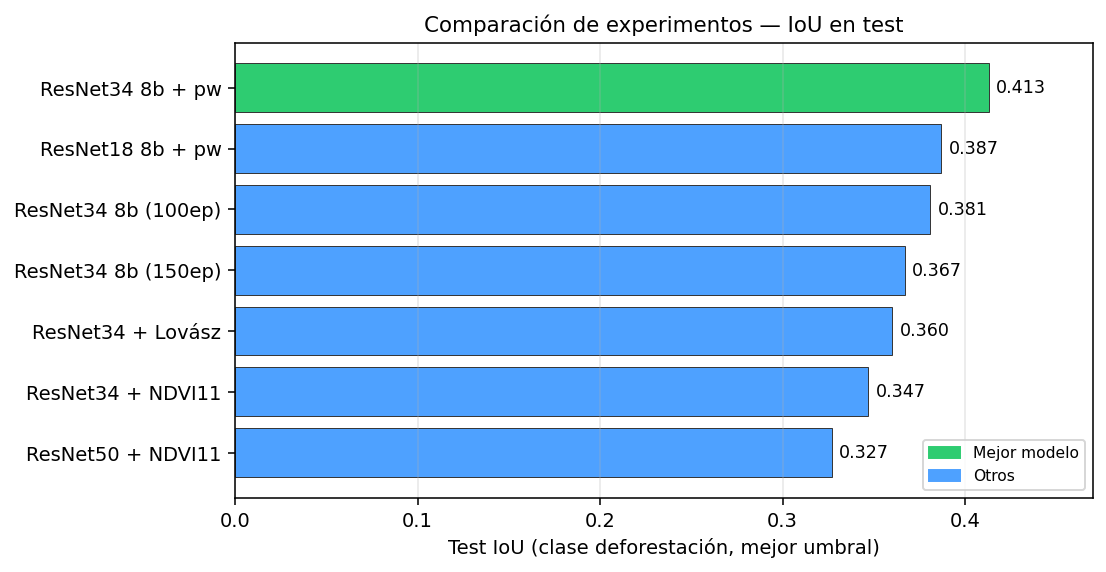
\includegraphics[width=0.92\textwidth]{figuras/comparacion_iou.png}
\caption{Comparación de la métrica IoU de prueba (con su mejor umbral) para los siete experimentos evaluados.}
\label{fig:comparacion}
\end{figure}

\begin{figure}[h]
\centering
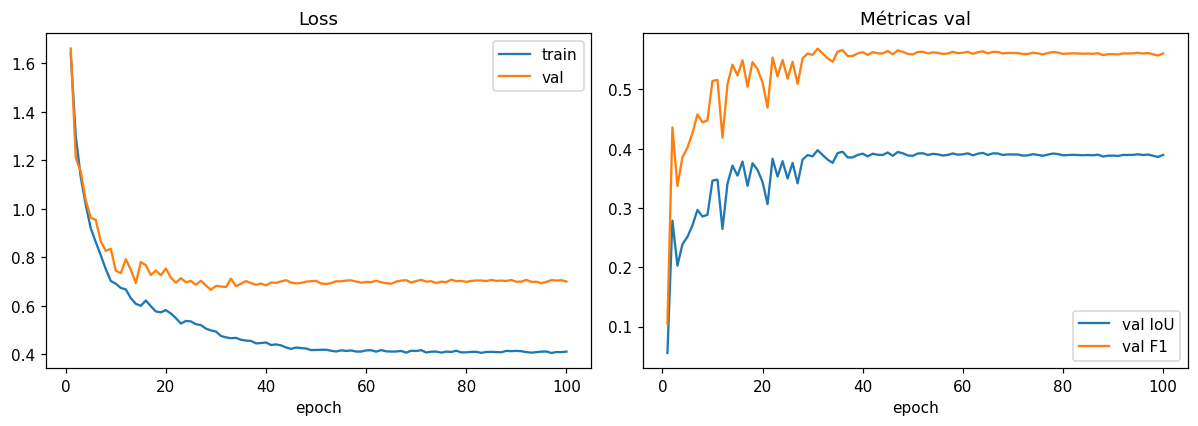
\includegraphics[width=0.92\textwidth]{figuras/curvas_mejor.png}
\caption{Curvas de entrenamiento de la mejor configuración (ResNet34 + 8 bandas + \texttt{pos\_weight} balanceado). Izquierda: pérdida de entrenamiento y validación. Derecha: IoU y F1 de validación a lo largo de las épocas.}
\label{fig:curvas}
\end{figure}

A continuación se analiza detalladamente el impacto de cada ajuste:

\paragraph{Tamaño del Encoder (ResNet18 vs ResNet34 vs ResNet50):}
Se observa que el rendimiento en términos de IoU sigue una curva de U invertida con respecto al número de parámetros del codificador:
\begin{itemize}
    \item \textbf{ResNet18 ($\sim$14M parámetros):} Obtiene un IoU de 0,387. La menor capacidad de la red causa un ligero subajuste (*underfitting*), limitando su capacidad de representar el cambio de cobertura de manera óptima.
    \item \textbf{ResNet34 ($\sim$24M parámetros):} Alcanza el máximo rendimiento con un IoU de 0,413. Representa el punto de equilibrio adecuado.
    \item \textbf{ResNet50 ($\sim$32M parámetros):} Cae drásticamente a un IoU de 0,327. Al disponer únicamente de 727 muestras de entrenamiento, la alta capacidad del codificador ResNet50 facilita que la red memorice las características particulares de las imágenes de entrenamiento (*overfitting*), en lugar de generalizar los patrones reales de deforestación.
\end{itemize}

\paragraph{Uso de Características Derivadas (NDVI como bandas extra):}
La incorporación de 3 canales extra con el cálculo explícito del NDVI antes, después y la diferencia temporal ($\Delta$-NDVI) para un total de 11 canales de entrada empeoró el desempeño ($0,413 \to 0,347$). Dado que el NDVI es una combinación matemática directa de las bandas R y NIR ($(\text{NIR}-\text{R})/(\text{NIR}+\text{R})$), la red es perfectamente capaz de calcular esta relación de forma interna en sus primeras capas convolucionales. Proporcionarlo explícitamente solo añade canales con pesos inicializados de forma aleatoria, introduciendo ruido y aumentando el sobreajuste sobre un dataset de tamaño limitado.

\paragraph{Peso de la Pérdida en la Clase Deforestación (\texttt{pos\_weight}):}
El ajuste de balance de clases mediante el peso positivo (\texttt{pos\_weight}) en la función de pérdida BCE representó la mejora individual más significativa de todo el estudio ($0,381 \to 0,413$). La relación nativa entre píxeles negativos y positivos en el dataset es de $\approx 33{,}6$, lo cual castiga fuertemente la omisión de píxeles positivos pero induce al modelo a sobre-predecir y marcar falsos positivos (obteniendo un recall alto de 0,77 pero una baja precisión de 0,40). Reducir este factor aplicando la raíz cuadrada ($\approx 5{,}8$) balanceó de forma efectiva la precisión (0,51) y el recall (0,67) del modelo, maximizando el IoU final.

\paragraph{Función de Pérdida Lovász vs Dice+BCE:}
La implementación de Lovász loss como una aproximación continua para la optimización directa del IoU no ofreció mejoras en la generalización (IoU de 0,360) y rompió la calibración del modelo. El modelo entrenado con Lovász concentró las probabilidades predichas en los extremos, perdiendo la suavidad y haciéndose altamente inestable ante cambios leves en el umbral de decisión, donde el IoU colapsaba fuera del umbral 0,5. En contraste, la pérdida Dice + BCE resultó mucho más robusta.

\paragraph{Duración del Entrenamiento (100 vs 150 épocas):}
El incremento a 150 épocas no aportó ganancias de desempeño. Las curvas de validación confirman que la convergencia y estabilización de la pérdida y el IoU ocurren entre las épocas 55 y 90, por lo que 100 épocas son suficientes.

\section{Resultados}
La configuración seleccionada como óptima fue la constituida por la U-Net con codificador \textbf{ResNet34}, entrenada con \textbf{8 canales base} durante \textbf{100 épocas} utilizando la pérdida combinada \textbf{Dice + BCE con \texttt{pos\_weight} balanceado} ($\approx 5{,}8$). 

En el conjunto de prueba independiente, este modelo obtiene un desempeño de:
\begin{itemize}
    \item \textbf{IoU en la clase deforestación:} 0,413 (umbral óptimo de 0,7).
    \item \textbf{F1-score:} 0,584.
    \item \textbf{Precisión:} 0,51.
    \item \textbf{Recall:} 0,67.
\end{itemize}
La estabilidad de la métrica IoU (que se mantiene en el rango de 0,403 a 0,413 para diferentes umbrales del barrido) demuestra la correcta calibración de las probabilidades de salida de la red.

\subsection*{Comparación Referencial con la Literatura}
Para contextualizar las métricas obtenidas, la Figura~\ref{fig:literatura} presenta una comparación con los resultados publicados por Torres et al. \cite{torres2021deforestation} en una tarea similar de detección de deforestación en la Amazonía usando imágenes Sentinel-2.

\begin{figure}[h]
\centering
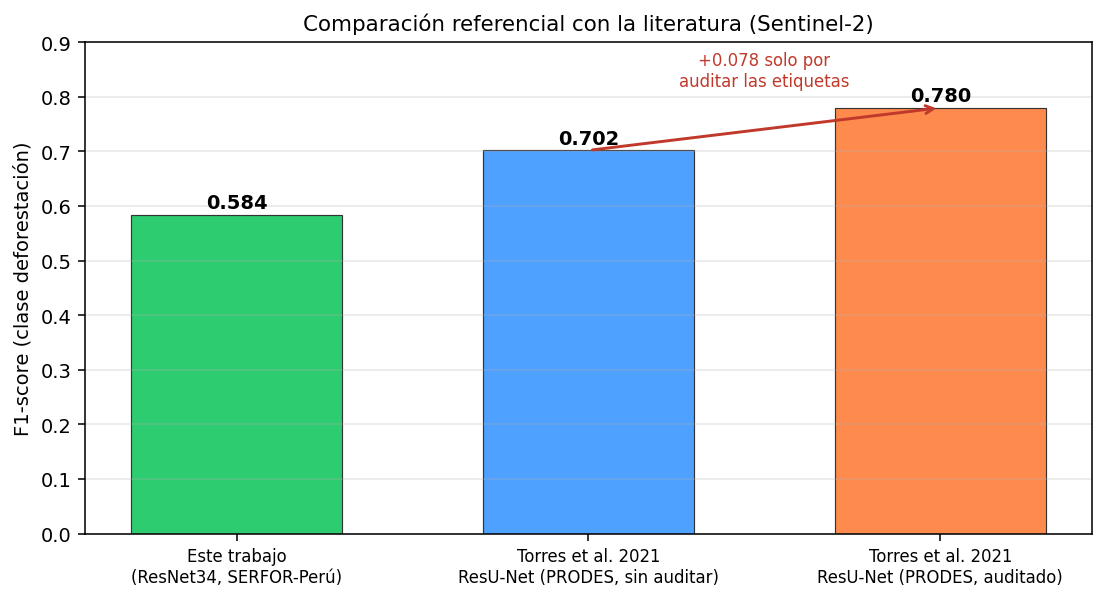
\includegraphics[width=0.92\textwidth]{figuras/comparacion_literatura.png}
\caption{Comparación referencial del F1-score de nuestro modelo frente al reportado por Torres et al. \cite{torres2021deforestation}. La comparación es de carácter cualitativo dada la diferencia en la escala de los conjuntos de datos y las etiquetas de referencia.}
\label{fig:literatura}
\end{figure}

El modelo ResU-Net propuesto por Torres et al. alcanza un F1-score de 70,2\% utilizando las etiquetas crudas del mapa PRODES de Brasil. Nuestro modelo obtiene un F1-score de 58,4\%. Esta brecha es razonable e inherente a las diferencias de escala: el estudio de Torres et al. cuenta con un volumen de datos masivo y continuo que cubre toda la Amazonía brasileña y etiquetas del sistema PRODES delineadas a escala fina, mientras que nuestro desarrollo se restringe a un conjunto limitado de 727 muestras de entrenamiento utilizando las etiquetas del portal oficial SERFOR de Perú.

\section{Limitaciones}
El principal factor limitante para la mejora del rendimiento métrico del modelo reside en la calidad intrínseca de los polígonos de referencia oficiales provistos por SERFOR. Estas etiquetas vectoriales fueron diseñadas con fines de catastro y reporte administrativo a escala gruesa, no para el entrenamiento de modelos de segmentación semántica a nivel de píxel. Frecuentemente presentan desplazamientos, delineaciones aproximadas y omisiones de áreas deforestadas reales adyacentes.

Dado que las métricas cuantitativas como el IoU se computan comparando pixel por pixel contra estas máscaras de referencia defectuosas, el IoU reportado está acotado artificialmente hacia la baja. De hecho, la inspección visual cualitativa del comportamiento del modelo revela que la red es capaz de identificar correctamente la deforestación en sus bordes reales, pero es penalizada cuantitativamente debido a que el polígono de referencia no se ajusta con exactitud a dicho contorno.

Adicionalmente, el reducido tamaño del dataset disponible tras el proceso de filtrado por nubes y solapamiento (727 pares para entrenamiento) restringe el uso de arquitecturas de mayor capacidad como ResNet50, propiciando el sobreajuste rápido si no se aplican técnicas estrictas de regularización y balance de pérdidas.

\section{Trabajo Futuro}
Con base en los resultados del estudio de ablación y las limitaciones identificadas, se proponen las siguientes líneas de trabajo:
\begin{itemize}
    \item \textbf{Curación masiva de datos:} Ampliar el proceso de edición y corrección manual de las máscaras a través del curador web interactivo desarrollado. Esta corrección fina de etiquetas representa la vía con mayor potencial de impacto para elevar el límite del IoU evaluado.
    \item \textbf{Incremento del volumen de entrenamiento:} Incorporar más escenas y pares de imágenes satelitales al dataset para mitigar los problemas de sobreajuste y permitir el entrenamiento de encoders más complejos.
    \item \textbf{Exploración de pérdidas alternativas:} Implementar y validar funciones de pérdida diseñadas específicamente para el desbalance de clases severo en segmentación de imágenes, como las pérdidas Tversky, Focal Tversky o pérdidas híbridas con regularización geométrica.
    \item \textbf{Análisis de errores localizado:} Analizar y categorizar de forma sistemática los fallos de predicción en las escenas de prueba que registran los peores IoU (identificando errores por presencia de coberturas nubosas residuales, sombras de nubes o áreas con firma espectral similar al suelo desnudo).
\end{itemize}

\section{Conclusiones}
A partir del desarrollo del sistema y los resultados del estudio de ablación, se desprenden las siguientes conclusiones principales:
\begin{enumerate}
    \item \textbf{El tratamiento del desbalance de clases es crucial:} El ajuste en la pérdida BCE usando el peso positivo balanceado (\texttt{pos\_weight} reducido a la raíz $\approx 5{,}8$) representó la mejora más importante de todo el estudio (elevando el IoU de 0,381 a 0,413), superando por mucho los efectos de cambios arquitectónicos.
    \item \textbf{Existe una relación clara de óptimo en la complejidad del encoder:} El rendimiento sigue una U invertida con respecto al tamaño de la red. ResNet18 resulta insuficiente (subajuste) y ResNet50 sobreajusta los datos debido a la escasez de muestras; ResNet34 constituye el punto de equilibrio óptimo para la cantidad de datos disponible.
    \item \textbf{Las características derivadas de forma manual no aportan valor:} Suministrar el NDVI calculado de forma explícita deteriora el rendimiento, debido a que el modelo puede aprender a calcularlo a partir de las bandas R y NIR nativas y el canal extra solo introduce ruido espectral.
    \item \textbf{La calidad de las etiquetas es el techo real del proyecto:} Tras optimizar los parámetros del entrenamiento, el limitante real no radica en el diseño de la red sino en la imprecisión de los polígonos SERFOR de referencia. La mejora de estas etiquetas mediante curación manual es fundamental para reportar métricas más realistas.
\end{enumerate}

% \section*{Agradecimientos}
% Agradecemos a la Universidad Nacional de Ingeniería (UNI) y a la Unidad de Posgrado de la Facultad de Ingeniería Industrial y de Sistemas (FIIS) por el soporte académico brindado en el desarrollo de este trabajo. Asimismo, extendemos nuestro agradecimiento al Servicio Nacional Forestal y de Fauna Silvestre (SERFOR) de Perú por proveer de forma abierta las bases de datos geográficas oficiales que sirvieron como punto de partida para este proyecto.

\bibliographystyle{plainnat}
\nocite{*}                  % Muestra todas las referencias aunque no estén citadas en el texto
\bibliography{referencias}

\appendix
\section*{Anexo: Contribución de los autores}
\begin{itemize}
    \item \textbf{Andrés Flores:} descarga y preprocesamiento de las imágenes Sentinel-2 vía STAC (notebook 02), filtrado por nubes y solapamiento, y armado del par \emph{antes/después}.
    \item \textbf{Víctor Lazo:} generación y rasterización de las máscaras a partir de los polígonos SERFOR (notebook 03), construcción del dataset de parches y partición por escena sin fuga de datos (notebook 04).
    \item \textbf{Rubén López:} diseño del pipeline y desarrollo del curador web \emph{before/after} para mejorar las etiquetas, e integración de las anotaciones manuales en las máscaras de entrenamiento.
    \item \textbf{Juan Quispe:} implementación y entrenamiento de la U-Net, estudio de ablación y análisis de los resultados (notebook 05).
\end{itemize}
Todos los autores participaron en la redacción, las pruebas y la corrección del manuscrito.

% \vspace{1em}
% \noindent\rule{\textwidth}{0.4pt}\\
% \footnotesize
% Artefactos por experimento en \texttt{data/experiments/<nombre>/} (checkpoint, curvas,
% \texttt{metrics.json}); tabla acumulada en \texttt{data/experiments/results.csv}.

\end{document}
